The gain achieved using the Oracular Patent Query method motivates us to explore various methods to approximate the terms
selected by this query without ``peeking at the answers'' provided by
the actual relevance judgements.  We first attempt this via fully
automated methods and then proceed to evaluate semi-automated methods
based on interactive relevance feedback methods.

\subsection{Automated Reduction}
\label{sec:AutomatedReduction}
%\vspace*{-2ex}
%We noticed that most of the useful feedback terms exist in the original query and hypothesized that the baseline system could be substantially improved by removing negative query terms. 
%
% Why these approaches? provide citations for who has suggested them or otherwise
% provide a justification as to why each approach would be a good idea.  Do this
% in the bullet points where the actual method is discussed... not after the bullet
% points!  Don't dissociate content and discuss it multiple times in different
% places!  -Scott
We use the following four simple approaches to reduce the initial Patent Query: 
%(i) removing Document Frequent terms (IDF(t)>$\tau$), (ii) keeping Frequent Terms in Query (QTF(t)>$\tau$); (iii) using Pseudo Relevance Feedback set (constructed after an initial run of the query) to select query terms (PRF(t)>$\tau$); and (iv) removing general terms in IPC title. 

\vspace*{0.5mm}
% TODO: Must be consistent in either pruning or removing terms --- results should ideally converge to the baseline at 0.
% TODO: Should do simplest comparisons first and not combine pruning approaches.  Even better: evaluate methods mentioned in related work.
\noindent \textbf{(i)} In standard IR approaches, removing terms appearing highly frequently across documents in the collection can improve retrieval effectiveness. Inspired by this fact, after an initial run of the query, we removed terms  with a high average document frequency (DF) over the top-100 documents ($\mathit{DF}(t)>\tau$). As seen in Figure \ref{fig:queryreduc} (magenta line), such pruning hurts performance. DF pruning continues increasing and converges to the baseline as $\tau \to \infty $ (i.e., no pruning).

\vspace*{0.5mm}
\noindent \textbf{(ii)} Frequent terms inside long and verbose queries are considered important~\cite{maxwell2013compact}. Thus, we hypothesize that removing terms appearing infrequently in the Patent Query may help and hence propose to remove terms with query term frequency (QTF) below a threshold $\tau$ ($QTF(t) \leq \tau$). Results in Figure~\ref{fig:queryreduc} (blue line) indicate the performance is slightly better than the baseline when removing low QTF terms.  The best MAP is achieved when $\tau=5$ and it meets the baseline when $\tau=0$ (i.e., all terms retained). 
%Frequent terms inside long and verbose queries have been shown to be important~\cite{maxwell2013compact}. Hence, we only keep high query TF (QTF) terms ($\mathit{QTF}(t)>\tau$) but remove from this set any document frequent terms ($\mathit{DF}(t)>0.01$). Figure \ref{fig:queryreduc} indicates that this approach performs slightly better than the baseline.

\vspace*{0.5mm}
\noindent \textbf{(iii)} We use Pseudo Relevance Feedback ($\mathit{PRF}$) to select query terms~\cite{maxwell2013compact} --- the same as we did for the Oracular Relevance Feedback system (Section~\ref{Sec:OracularTermSelection}). We assume that the top 5 retrieved documents are relevant and the rest are irrelevant (this performed best), then we calculate $\mathit{PRF}$ score based on this assumption.  
Terms that have $\mathit{PRF}$ score higher than the threshold $\tau$ ($PRF(t)>\tau$), are selected from the Patent Query to reformulate a reduced query. Figure~\ref{fig:queryreduc} (red line) shows that this approach is also unsuccessful at achieving a notable improvement over the baseline.

%The third query reduction approach is to select query terms using pseudo-relevance feedback ($\mathit{PRF}$)
%~\cite{Baeza-Yates2011, maxwell2013compact}. We calculated a $\mathit{PRF}$ score similar to $\mathit{RF}$ score assuming that the top-k ranked documents are relevant. We selected the query terms which have high $\mathit{PRF}$ score ($\mathit{PRF}(t)>\tau$). As Figure \ref{fig:queryreduc} illustrates, this approach does not notably outperform the baseline. 
%In fact, we could not find any heuristic correlation between  $ PRF(t)$ and $ RF(t)$. 

\vspace*{0.5mm}
\noindent \textbf{(iv)} The titles of IPC codes indicate the intended content of patents classified under that code by using a single phrase or several related phrases linked together. We used words in IPC code titles for each patent query as stopwords to reduce the query, based on the assumption that these terms are common to all patents having the same IPC code label.  As it can be seen in Figure~\ref{fig:queryreduc} (black line), this approach slightly helps the performance.
%Finally, we used words in IPC title of each patent query to reduce the query, based on the assumption they are common to all patents, which belong to the same category and may be considered as stop-words. In our experiment, we removed the IPC title terms from a selection of frequent query terms ($QTF(t)>5$). We can see in Figure \ref{fig:queryreduc} that the results drop slightly compared to approach (2), where $\tau=5$.
%\noindent \textbf{(1)-} In standard IR approaches, removing terms, appearing a lot in the collection, helps the retrieval effectiveness. Inspired by this fact, after an initial run of the query, we removed terms  with a Document Frequency (DF) in top-100 documents, higher than the threshold $\tau$. However, as illustrated in Figure \ref{fig:queryreduc}, it's clear that this technique significantly hurts the performance ($DF(t)>\tau$).  
%
%\noindent \textbf{(2)-} Intuitivelly, frequent terms inside long and verbose queries are  important~\cite{maxwell2013compact}. Hence, we have  choosen to reduce queries by selecting terms with a frequency higher than a certain threshold $\tau$. The results in Figure \ref{fig:queryreduc} indicate clearly that this simple and naive technique is not adequate ($QTF(t)>\tau$). 
%
%\noindent \textbf{(3)-} The third approach we experiment to reduce the query is based on Pseudo Relevance Feedback ($\mathit{PRF}$)~\cite{Baeza-Yates2011}. $\mathit{PRF}$ is an automated process without user interaction, which assumes the top k ranked documents are relevant. Again, it can be seen in Figure \ref{fig:queryreduc} that the results for query reduction using $\mathit{PRF}$ do not notably outperform the baseline. In fact, we could not find any heuristic correlation between  $ PRF(t)$ and $ RF(t)$. 
%%Reda: Need clearly to be explained!}
%
%\noindent \textbf{(4)-} Finally, we used words in IPC code title of each patent query to reduce the query, based on the assumption that they are common to all patents, which belong to the same category and may be considered as stop-words. However it did not help.

%we hurt the effectiveness by filtering them out.

% The anecdotal results and their implications have to be explained
% much more clearly... what is surprising about them (be specific:
% point out actual terms) and what can you take away from this
% investigation.  -Scott
\vspace*{0.5mm}
% TODO: What is an IPC title?  I don't know that this is... was it discussed?
Figure \ref{fig:anecdotal} shows an anecdotal example for a sample query about an invention related to ``emulsifier'' to help explain why these four approaches \emph{fail}. It shows the raw abstract of the invention, and the top 20 high-scoring terms (except for IPC Title Terms which are not scored, but simply displayed) and their associated $\mathit{RF}$ scores for each approach. 
% Scott: the following is unclear... instead have modified Figure 3 caption.
%IPC title terms are the words appearing in the IPC title and do not have any score.
%\begin{displaymath}\{t| DF(t)/QTF(t)/PRF(t)>10\}\end{displaymath}
It can be seen that the four methods fail to clearly discriminate between useful and noisy terms.  Important stemmed terms like ``enzym'' and ``starch'' would be pruned according to DF; in contrast, QTF and PRF both score ``starch'' highly and retain it, but also retain other noisy terms.  Over half of the IPC Title Terms are noisy and appropriate to remove, but critical useful stemmed terms like ``emulsifi'' are also removed.
%As one example, important stemmed terms like ``enzym'' and ``starch'' have been removed by the DF pruning approach, which hurts query quality.  As another example, pruning IPC title terms removes highly noisy (negative) terms like ``amylos'' or ``saccharid'', but also removes useful terms like ``emulsifi''.  
%pruning IPC title terms yields more noisy terms than useful terms (13 out of 20 terms were noisy and removed, but more rare negative terms like ``amylos'' or ``saccharid'' remain).
  Critically, all methods retain noisy terms (red/negative) and results from Section~\ref{sec:baseline_vs_oracular} showed that the inclusion of even slightly noisy terms can significantly hurt performance.  Overall, all methods fail to retain only the oracular query terms (blue/positive) and do worse than PATATRAS.
%which resulted in bad retrieval performance. 
%Therefore, this may suggest more sophisticated query reduction methods, as the one discussed in the next section.
 

%high scored terms are polluted with the sufficient amount of noise to hurt the retrieval effectiveness. Unfortunately, none of the proposed query reduction approaches for query reduction worked better than the baseline, which leads us to investigate interactive methods for reduction in the next section.

\subsection{Semi-automated Interactive Reduction}

\label{sec:SemiAutomatedInteractiveReduction}

%%%%%%%%%%%%%%%%%%%%%%%%%%%%%%%%%%%%%%%%%%%%%%%%%%%%%%%%%%%%
%\begin{figure}[t!]
%\begin{centering}
%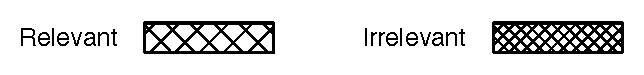
\includegraphics[width=9cm]{imgs/legend2}
%\par\end{centering}
%
%\begin{centering}
%\subfigure[{Mean Average Precision.}]{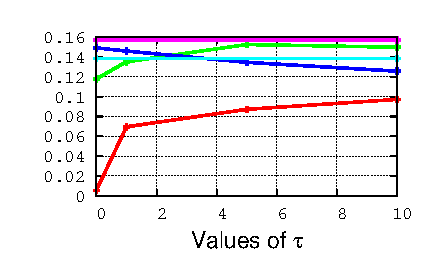
\includegraphics[width=4.5cm]{imgs/figure2-MAP}}\subfigure[Recall.]{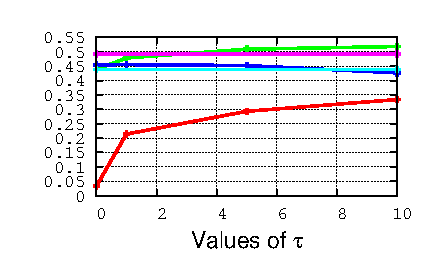
\includegraphics[width=4.5cm]{imgs/figure2-Recall}}
%\par\end{centering}
%
%\protect\caption{System performance vs. the threshold $\tau$ for four query reduction approaches.}
%\label{fig:queryreduc}
%\end{figure}
%%%%%%%%%%%%%%%%%%%%%%%%%%%%%%%%%%%%%%%%%%%%%%%%%%%%%%%%%%%%
%%%%%%%%%%%%%%%%%%%%%%%%%%%%%%%%%%%%%%%%%%%%%%%%%%%%%%%%%%%%
\begin{figure}[t!]
\begin{centering}
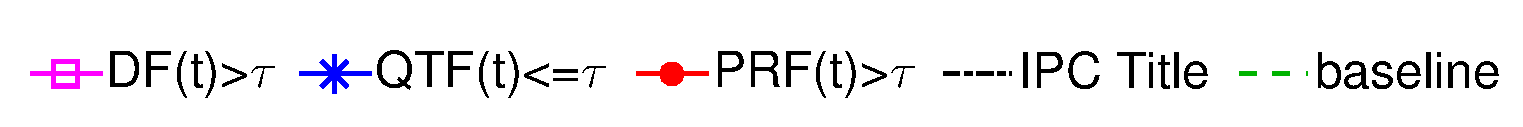
\includegraphics[width=9cm]{imgs/l2.eps}
\vspace*{-4ex}
\par\end{centering}
\begin{centering}
\subfigure[{Mean Average Precision.}]{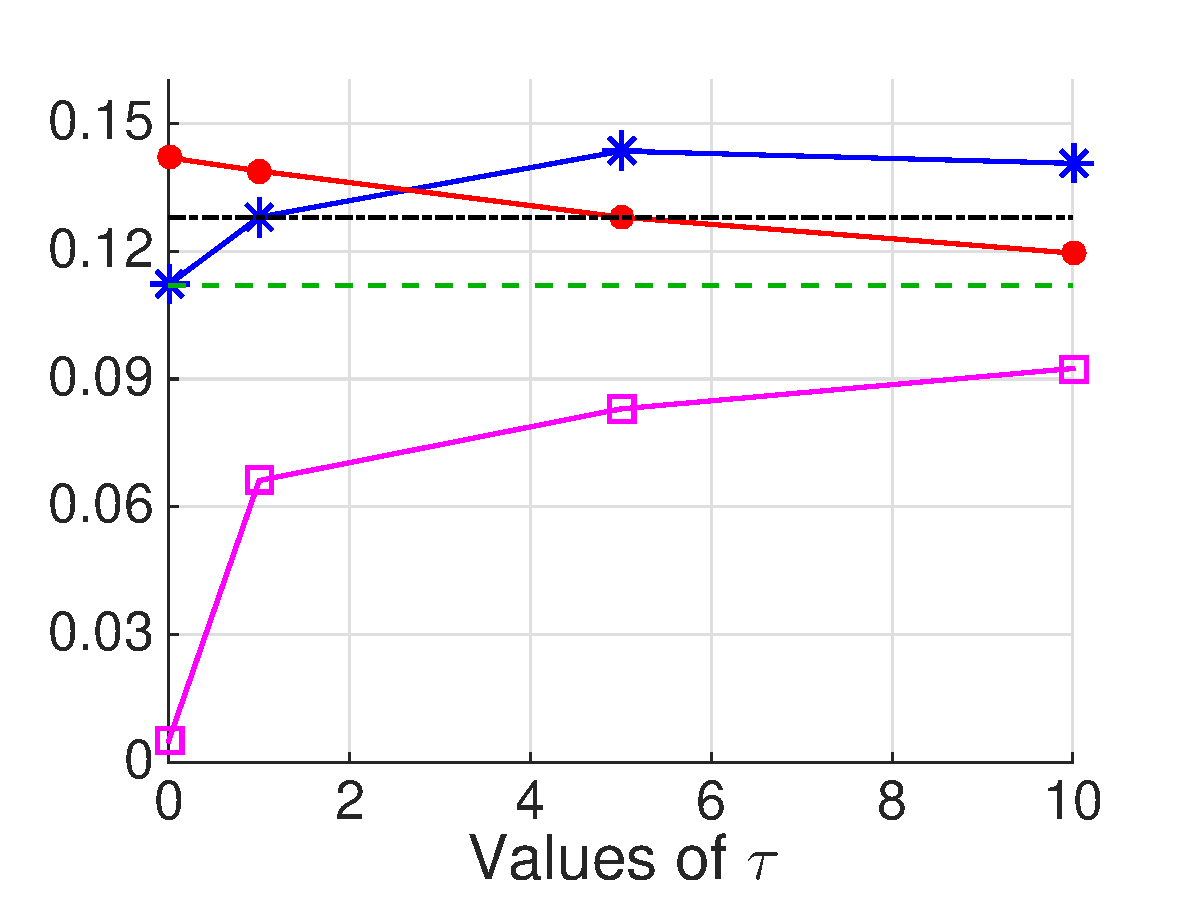
\includegraphics[width=4.5cm, height=3.5cm]{imgs/fig2_map_cr}}\subfigure[Recall.]{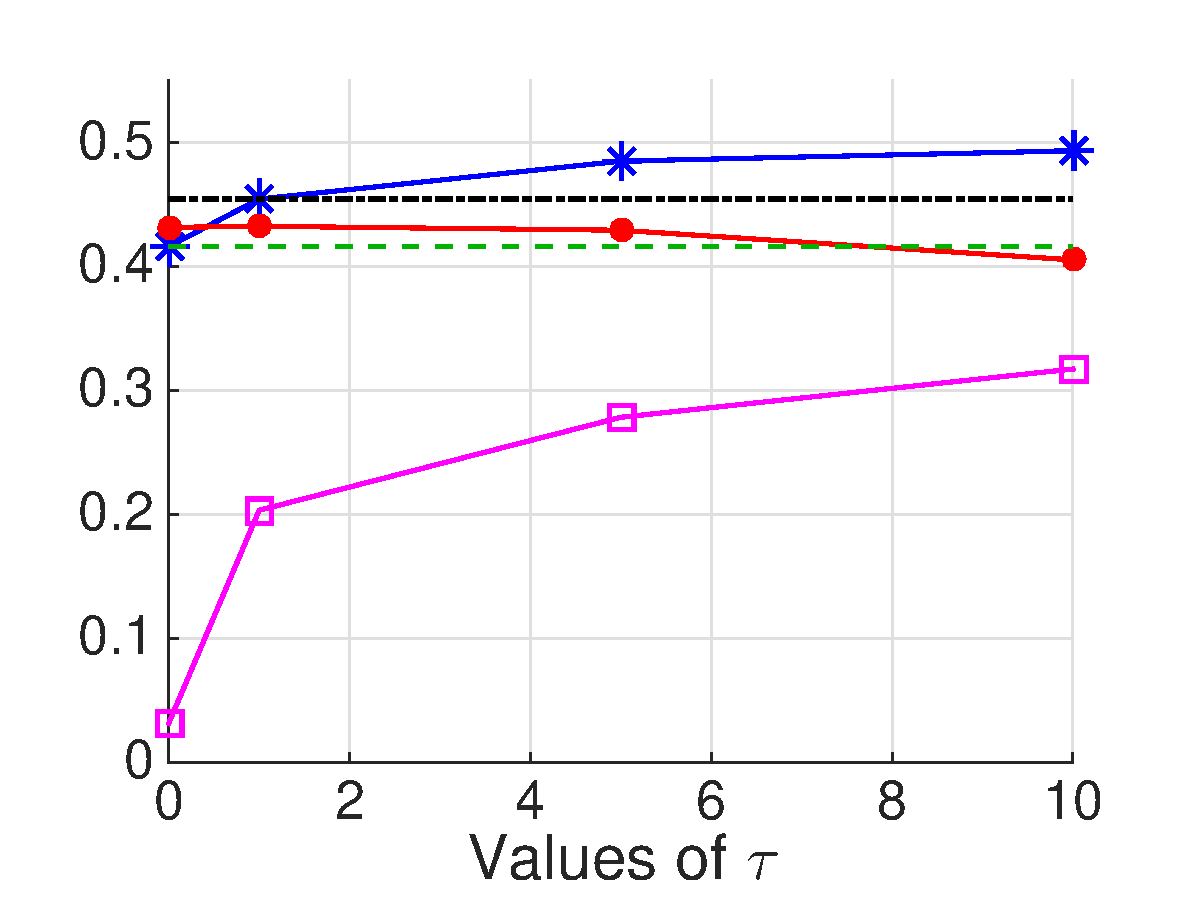
\includegraphics[width=4.5cm, height=3.5cm]{imgs/fig2_recall_cr}}
\par\end{centering}
\vspace*{-2ex}
\protect\caption{System performance vs. the threshold $\tau$ for four query reduction~approaches.}
\label{fig:queryreduc}
\end{figure}
%%%%%%%%%%%%%%%%%%%%%%%%%%%%%%%%%%%%%%%%%%%%%%%%%%%%%%%%%%%%
%%%%%%%%%%%%%%%%%%%%%%%%%%%%%%%%%%%%%%%%%%%%%%%%%%%%%%%%%%%%
\begin{figure}[t!]
\begin{framed}
\vspace*{-2ex}
  \centering
    %\lstinputlisting[frame=single, basicstyle=\scriptsize\ttfamily , linewidth=\columnwidth,breaklines=true]{code/anecdotale.tex}\vspace*{-2ex}
 \begin{lstlisting}[basicstyle=\scriptsize\ttfamily , linewidth=\columnwidth,breaklines=true] 
(PAC-1293) - Abstract: The invention relates to an 
emulsifier, a method for preparing said emulsifier, 
and to its use in various applications, primarily 
food and cosmetic applications.The invention also 
relates to the use of said emulsifier for the 
creation of an elastic, gelled foam.  An emulsifier 
according to the invention is based on a starch 
which is enzymatically converted, using a specific 
type of enzyme, and modified in a specific 
esterification reaction.
<@\vspace{-2mm}@>
<@\underline{DF Terms:}@><@\textcolor{blue}{starch:14.6}@>,<@\textcolor{blue}{enzym:29.5}@>,<@\textcolor{red}{amylos:-20.1}@>,<@\textcolor{blue}{oil:8.6}@>,
<@\textcolor{red}{dispers:-8.7}@>,<@\textcolor{red}{ph:-4.6}@>,<@\textcolor{red}{dry:-6.2}@>,<@\textcolor{red}{heat:-2.3}@>,<@\textcolor{red}{product:-5.5}@>,
<@\textcolor{red}{slurri:-11}@>,<@\textcolor{blue}{viscos:8}@>,<@\textcolor{red}{composit:-4}@>,<@\textcolor{red}{reaction:-2}@>,<@\textcolor{red}{food:-12}@>,
<@\textcolor{blue}{agent:5}@>,<@\textcolor{red}{debranch:-11}@>,<@\textcolor{red}{reduc:-6}@>,<@\textcolor{red}{fat:-13}@>,<@\textcolor{red}{prepar:-0.8}@>,
<@\textcolor{red}{hour:-5}@>
<@\vspace{-2mm}@>
<@\underline{QTF Terms:}@><@\textcolor{blue}{starch:14.6}@>,<@\textcolor{blue}{emulsifi:6.7}@>,<@\textcolor{red}{succin:-3.5}@>,
<@\textcolor{blue}{enzym:29.5}@>,<@\textcolor{blue}{emuls:12.7}@>,<@\textcolor{blue}{hydrophob:5.4}@>,<@\textcolor{red}{anhydrid:-5.5}@>,
<@\textcolor{red}{reaction:-2}@>,<@\textcolor{red}{octenyl:-0.7}@>,<@\textcolor{blue}{stabil:3.6}@>,<@\textcolor{blue}{alkenyl:0.06}@>,
<@\textcolor{blue}{reagent:1.2}@>,<@\textcolor{blue}{carbon:0.1}@>,<@\textcolor{blue}{potato:3.7}@>,<@\textcolor{red}{alkyl:-0.3}@>,<@\textcolor{red}{wt:-4.6}@>,
<@\textcolor{blue}{ether:2}@>,<@\textcolor{red}{enzymat:-3.4}@>,<@\textcolor{blue}{convers:10.4}@>,<@\textcolor{red}{chain:-5.5}@>
<@\vspace{-2mm}@>
<@\underline{PRF Terms:}@><@\textcolor{blue}{starch:14.6}@>,<@\textcolor{blue}{encapsul:17.5}@>,<@\textcolor{red}{chees:-4}@>,<@\textcolor{blue}{oil:8.6}@>,
<@\textcolor{blue}{hydrophob:5.4}@>,<@\textcolor{blue}{agent:5}@>,<@\textcolor{red}{casein:-2.2}@>,<@\textcolor{blue}{degrad:17}@>,<@\textcolor{blue}{deriv:12}@>,
<@\textcolor{blue}{tablet:5.3}@>,<@\textcolor{red}{debranch:-11}@>,<@\textcolor{red}{imit:-1}@>,<@\textcolor{blue}{viscos:7.8}@>,<@\textcolor{blue}{oxid:6}@>,
<@\textcolor{blue}{activ:6}@>,<@\textcolor{blue}{osa:9.3}@>,<@\textcolor{blue}{funnel:2.7}@>,<@\textcolor{blue}{amylas:26}@>,<@\textcolor{red}{amylopectin:-7}@>,
<@\textcolor{blue}{maiz:20.6}@>
<@\vspace{-2mm}@>
<@\underline{IPC Title Terms:}@><@\textcolor{blue}{cosmet:3.8}@>,<@\textcolor{blue}{toilet:0.2}@>,<@\textcolor{red}{prepar:-0.8}@>,
<@\textcolor{blue}{case:0.5}@>,<@\textcolor{red}{accessori:-0.01}@>,<@\textcolor{red}{store:-0.4}@>,<@\textcolor{blue}{handl:0.07}@>,
<@\textcolor{red}{pasti:-0.2}@>,<@\textcolor{red}{amylos:-20}@>,<@\textcolor{red}{fibrou:-0.01}@>,<@\textcolor{red}{pulp:-1.3}@>,
<@\textcolor{red}{constitut:-0.06}@>,<@\textcolor{blue}{paper:1.3}@>,<@\textcolor{red}{impregn:-0.1}@>,<@\textcolor{blue}{emulsifi:6.7}@>,
<@\textcolor{red}{wet:-0.3}@>,<@\textcolor{red}{dispers:-9}@>,<@\textcolor{red}{saccharid:-12}@>,<@\textcolor{red}{produc:-0.6}@>,<@\textcolor{blue}{agent:5}@>
 \end{lstlisting} 
 \vspace*{-3ex}
\end{framed}
 \vspace*{-3.5ex}
  \caption{The top 20 terms scored by each of four methods on a sample
    query (except for IPC Title Terms which are not scored); whether the term is
    pruned or retained depends on the approach, cf. (i)--(iv).
    Numerical oracular scores $\mathit{RF}(t,Q)$ are provided
    indicating whether the term was actually useful (blue/positive) or
    noisy (red/negative).}
  \label{fig:anecdotal}  
 \vspace*{-1.5ex}
\end{figure}
%%%%%%%%%%%%%%%%%%%%%%%%%%%%%%%%%%%%%%%%%%%%%%%%%%%%%%%%%%%%

Our sample analysis of specific queries and terms selected via our oracular
approach suggests that automated methods fall far short of optimal term selection.
This leads us to explore another approach of approximating the oracular query
derived from relevance judgements by using a subset of relevance judgements
through interactive methods.  Specifically, to evaluate the impact of minimal user interaction,
\textcolor{black}{we next analyze the performance of an Oracular Patent Query (Equation \ref{eq:score}) derived from
\emph{only} the top-$k$ ranked relevant documents identified in the search results (for small $k$) --- we assume that the remaining documents in the top-100 are irrelevant.}
\begin{comment}
All our attempts to improve the system effectiveness without accessing the relevance feedback were quite in vein because the features we recognized were tightly the combination of the useful words and noisy words and the system performance is too sensitive to the existence of a noisy word or the absence of the useful terms. So, we decided to apply much more realistic approach in which feedback terms are extracted only from the first ranked relevant document retrieved. 
\end{comment}
Using this approach, Table \ref{tab:firstrel} shows that we can double the MAP in comparison to our baseline and also outperform the PATATRAS system by identifying only the \emph{first} relevant document.
%%%%%%%%%%%%%%%%%%%%%%%%%%%%%%%%%%%%%%%%%%%%%%%%%%%%%%%%%%%%%%%%
\begin{table}[t!]
  \begin{center}
   \caption{System performance using minimal relevance feedback. $\tau$ is RF score threshold, and $k$ indicates the number of top relevant patents.}\vspace{3mm}
  \input table/table2-cr.tex   
  \label{tab:firstrel}
  \end{center}  
\end{table}
%%%%%%%%%%%%%%%%%%%%%%%%%%%%%%%%%%%%%%%%%%%%%%%%%%%%%%%%%%%%%%%%

Furthermore, to establish the minimal interaction required by this
approach, Figure \ref{fig:FirstTPRankHisto} indicates that the
baseline methods return a relevant patent approximately 80\% of the
time in the first 10 results and 90\% of the time in the first 20
results. Hence, such an interactive approach requires relatively low
user effort while achieving state-of-the-art performance.


\begin{figure}
\vspace{-2mm}
\begin{centering}
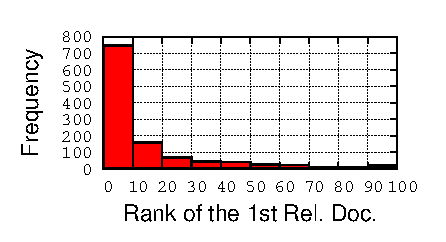
\includegraphics[width=5.5cm]{imgs/1stRank}
\par\end{centering}

\protect\caption{The distribution of the first relevant document rank over test queries.  
%Clearly, the first relevant document is often found in the top-20 meaning that it can identified without excessive search.
}
\label{fig:FirstTPRankHisto}
\vspace{-1mm}
\end{figure}


